%%%%%%%%%%%%%%%%%%%%%%%%%%%%%%%%%%%%%%%%%%%%%%%%%%%%%%%%%%%%%%%%%%%%%%%%
% Plantilla TFG/TFM
% Escuela Politécnica Superior de la Universidad de Alicante
% Realizado por: Jose Manuel Requena Plens
% Contacto: info@jmrplens.com / Telegram:@jmrplens
%%%%%%%%%%%%%%%%%%%%%%%%%%%%%%%%%%%%%%%%%%%%%%%%%%%%%%%%%%%%%%%%%%%%%%%%

\chapter{Estado del arte}

\section{La demoscene}

\subsection{Qué es la demoscene}

La \emph{demoscene} es una subcultura informática cuyo principal objetivo es la creación de demostraciones técnicas llamadas \emph{demoscenes}. Una \emph{demoscene} es un programa autocontenido y por norma general de peso ligero que intenta explotar al máximo el \emph{software} y el \emph{hardware} de la máquina que la ejecuta, con el fin de generar efectos visuales y sonoros. El objetivo de una \emph{demoscene} suele consistir en mostrar el ingenio y las habilidades del programador, así como tratar de impresionar al público.\\

Además, aunque el \emph{demoscening} en sí mismo no se puede considerar una forma de arte, sí que es cierto que muchas demos poseen un cierto componente artístico.\\ 

Se distinguen principalmente dos tipos de demo\footnote{\url{http://www.oldskool.org/demos/explained/demo_reference.html}}:

\begin{itemize}
  \item \textbf{Demo}: programa que genera gráficos y sonido en tiempo real. Suele tener una extensión superior a 5 minutos y normalmente no tienen límite de tamaño. Una demo suele ser creada por un grupo de personas que incluye al menos un programador, un diseñador gráfico y un músico. Las demos actuales suelen estar realizadas en 3D y cuentan con aceleración gráfica por hardware. Las demos más antiguas o realizadas para plataformas más antiguas (conocidas como "demos \emph{oldskool}") son procesadas de forma íntegra por la CPU (pues las plataformas para las que se desarrollan no poseen GPU) y suelen combinar ilusiones 3D con efectos gráficos en 2D.
  \item \textbf{Intro}: una demo de corta duración. Una intro suele ser temática (mientras que una demo suele compilar distintas escenas/temáticas). Además, las intros no suelen superar los 5 minutos de duración y su tamaño tiende a estar restringido. Las principales categorías de intros son 64K (65536 bytes), 4K (4096 bytes) y 1K (1024 bytes).
\end{itemize}

Existen otras categorías de demo, aunque son mucho menos comunes, como las \textbf{mega demos} (demos de gran duración/extensión, compuestas por múltiples partes) o las \textbf{dentros} (intros cuyo propósito es ofrecer un avance de una demo por llegar, todavía en desarrollo).\\

Además, existen muchas otras categorías derivadas o relacionadas con la \emph{demoscene}, como la creación de gráficos procedurales. Una de las subcategorías más populares dentro de esta son las \textbf{4K images}, imágenes complejas y de alta resolución generadas proceduralmente por programas de 4096 bytes. También es posible encontrar categorías similares relacionadas con la generación procedural de archivos de música o vídeo. Las mayores diferencias entre estas producciones y las demos son su tiempo de ejecución (no se ejecutan en tiempo real) y las técnicas que usan (al no ser el tiempo una limitación, pueden usar algoritmos computacionalmente más costosos, pero que generan resultados más complejos).

\subsection{Orígenes de la demoscene}

A principios de los años 80, con la popularización de los primeros ordenadores personales, la computación dejó de ser algo que sucedía en universidades para pasar a abrirse al gran mercado. Con ello, llegó también la distribución del software, aunque en aquella época no se producía por internet, si no tan sólo por medios físicos, como los disquetes. Estos programas venían con protecciones de copia por parte de los desarrolladores para evitar su distribución ilegal. Poco tardaron, no obstante, en aparecer los primeros \emph{crackers}, personas que se dedicaban a eliminar las protecciones de copia del software para su distribución gratuita. Esto llevó a la creación de una subcultura informática basada en el \emph{cracking} de videojuegos y otros tipos de software, al margen de la legalidad. Esto se hacía no solo con la intención de poder ditribuir el software de forma gratuita, si no que también suponía una fuente de diversión y competición para los \emph{crackers}\footnote{\url{https://web.archive.org/web/20170726063815/http://tomaes.32x.de/text/faq.php\#2.3}}.\\

Es por ello que los denominados \emph{crackers} empezaron a "firmar" el software que \emph{crackeaban} con seudónimos que aparecían en los menús o en las intros de los juegos. Con el tiempo, la competición y la ambición de los \emph{crackers} fue aumentando, y llegó un punto en el que no solo se limitaban a quitar las protecciones de copia del software, si no que también creaban sus propias intros para los programas.\\

Es en este punto cuando la \emph{demoscene} empieza a tomar forma, cuando una parte de los \emph{crackers} deciden retornar a la legalidad pero sin dejar atrás la competición y la diversión. De este modo, este nuevo sector se empieza a dedicar a la creación de intros y demos cuyo objetivo es mostrar sus habilidades al resto de \emph{demosceners}\footnote{\url{http://widerscreen.fi/assets/reunanen-wider-1-2-2014.pdf}}.

\subsection{Composición y cultura de la demoscene}

La \emph{demoscene} es una subcultura informática muy centrada en el trabajo en equipo y en compartir. Con el desarrollo y popularización de la \emph{demoscene}, a partir de principios de los 90 se popularizó y se estandarizó, con la creación de eventos y competiciones.\\

Heredado de las \emph{copyparties}, eventos en los que \emph{crackers} y \emph{demosceners} se juntaban para conocerse y compartir software, al margen de la legalidad, nuevos eventos empezaron a crearse a principios de los noventa. Estos eventos sí eran legales y se centraban únicamente en el aspecto de las demos. Pasan a ser eventos sociales en los que los \emph{demosceners} se conocen, comparten y compiten.\\

Estos eventos, conocidos como \emph{demoparties}, pasan entonces a ser concursos y tener distintas categorías y premios. Para concursar, normalmente los competidores se juntaban en grupos, usualmente compuestos por al menos un programador, un diseñador gráfico y un músico. Estos grupos tenían su propio nombre e identidad. A su vez, cada uno de los componentes del grupo también solía usar un seudónimo. El uso de un seudónimo es una herencia de los orígenes de la \emph{demoscene} en el \emph{cracking}, aunque el propósito de usar un alias cambia. Mientras que los \emph{crackers} usaban un nombre falso para ocultar su identidad, pues realizaban actividades ilegales, los \emph{demosceners} usan este alias como una forma de expresión.

\subsection{La demoscene en la actualidad}

Si bien la \emph{demoscene} siempre se ha mantenido como una subcultura y nunca ha llegado a tener una popularidad masiva, su auge se dio en los años noventa.  En la actualidad, muchos de los eventos de \emph{demoscening} que se crearon en los 90 han desaparecido, y otros tantos han derivado en eventos dedicados a los ordenadores de forma mucho más genérica, derivando en eventos de software o en \emph{LAN-parties}.\\

Del mismo modo que muchas ferias y eventos han desaparecido, muchos otros también se han ido creando. No obstante, parece que hay una tendencia general hacia el olvido.\\

Las \emph{demoparties} en la actualidad suelen ser eventos locales, normalmente humildes, donde participan apasionados y nostálgicos.\\

Es difícil atribuir las causas de la lenta caída en popularidad de la \emph{demoscene}, aunque hay varios factores que pueden contribuir a ello, del mismo modo que hay una serie de factores que evitan que se pierda.\\

Por un lado, la \emph{demoscene} es cada vez más pequeña debido a:

\begin{itemize}
  \item Siempre ha sido una subcultura, y nunca ha destacado especialmente por encima de otras subculturas informáticas.
  \item Para poder participar en la \emph{demoscene} hace falta una gran cantidad de conocimiento matemático y de programación de bajo nivel, cualidades que no abundan.
  \item Con el auge de los ordenadores, otro tipo de espacios más accesibles al público como las ferias tecnológicas, las ferias de videojuegos o las ferias de programación han eclipsado parcialmente a la \emph{demoscene}.
  \item Una parte de los \emph{demosceners} eran reacios a la incorporación de gente nueva e inexperta a la \emph{demoscene}, pues si bien aportaban sangre nueva, sus metas y conocimiento se alejaban de los originales de la escena.
\end{itemize}

Todos estos factores han contribuido a colocar la \emph{demoscene} como una práctica de nicho. Quizá una crítica válida sería que no ha sabido adaptarse de forma conveniente a los nuevos tiempos. El mundo de la \emph{demoscene} no ha sabido publicitarse o venderse suficientemente bien como para llegar a ser conocido por un público mayor. Sin embargo, la \emph{demoscene} sigue viva, y estos son algunos de los factores que contribuyen a ello:

\begin{itemize}
	\item El auge de lo \emph{retro}. En esta última década ha empezado a masivizarse un cierto reconocimiento y nostalgia hacia los orígenes de la computación y del videojuego. La popularización de los juegos \emph{indie}, técnicas como el \emph{pixel art} y tributos a videojuegos antiguos han llevado a destapar obras olvidadas y a suscitar un nuevo interés por todo lo \emph{retro}.
	\item La pasión y dedicación de los \emph{demosceners}, que siguen produciendo y compartiendo su obra, extendiendo así su pasión y abriéndola al público general.
	\item La masivización de la informática. Hoy en día hay muchísimos más informáticos que en los años 80 y 90. Si bien es cierto que hay una tendencia de abandono hacia el bajo nivel, también hay mucha más gente que se hace preguntas, investiga y se interesa por el mismo.
\end{itemize}

Como reflexión final me gustaría añadir que creo que es posible mantener el panorama de la \emph{demoscene} vivo, pero pienso que esto va a ser muy complicado si no se intenta abrir al público, cosa que algunas \emph{demoparties} ya están haciendo. Está claro que al abrir la \emph{demoscene} al público general se pierden cosas por el camino, y se gana gente que tiene un interés mucho más casual y mucho menos pasional. Creo que en el panorama actual esa gente es necesaria. No todo el mundo tiene el tiempo o la capacidad como para meterse de lleno en la \emph{demoscene}, pero hay muchas personas que sí pueden tener curiosidad por ella de una forma mucho más básica, y esta gente también cuenta. Cada vez es más común encontrar en ferias de videojuegos puestos \emph{retro}, y hay incluso museos del videojuego. La nostalgia y la veneración por los orígenes se abre paso, y pienso que es en este lugar donde la \emph{demoscene} puede buscar su camino.

\section{Eventos de demoscening}

A continuación se listan y describen brevemente algunas \emph{demosparties} que aún se celebran en la actualidad, en el año 2019.

\begin{itemize}
	\item \textbf{Revision}: tiene lugar en durante Pascua, en Alemania. Es la sucesora de la \emph{demoparty} Breakpoint\footnote{\url{http://breakpoint.untergrund.net}}. El evento se estableció en 2011, tras el fin de Breakpoint, y mantiene a muchos de los organizadores. El evento congrega a más de 800 personas de todo el mundo cada año, y es el mayor evento dedicado exclusivamente a la \emph{demoscene} en el mundo \footnote{\url{https://2019.revision-party.net}}.
	\item \textbf{Assembly}: tiene lugar en verano en Finlandia, y es el mayor evento de \emph{demoscening} en el país. Además, es uno de las \emph{demoparties} más antiguas que siguen en activo, cumpliendo 25 años el pasado 2017. Sin embargo, el evento no está dedicado exclusivamente a la \emph{demoscene}, si no que es también un evento de videojuegos y \emph{esports}. No obstante, la \emph{demoscene} sigue siendo importante en él, y se celebran anualmente concursos en 5 categorías distintas (Demo, Oldskool demo, 64K intro, 4K intro y 1K intro)\footnote{\url{https://www.assembly.org/summer19/demoscene}}.
	\item \textbf{VIP (Very Important Party)}: es la \emph{demoparty} más longeva de Francia, cumpliendo este año su 20 aniversario. Congrega a personas de todas partes de Europa, aunque es una \emph{demoparty} principlamente francesa\footnote{\url{https://en.wikipedia.org/wiki/Very_Important_Party}}. Fue fundada por el grupo de \emph{demosceners} \emph{PoPsY TeAm}\footnote{\url{http://www.popsyteam.org}}.
	\item \textbf{Nova}: esta \emph{demoparty} fue creada en 2017, por lo que este año se celebra su tercera edición. Es la mayor \emph{demoparty} en Reino Unido, con una salón principial con capacidad para hasta cien \emph{demosceners}\footnote{\url{http://www.novaparty.org}}.
	\item  \textbf{Alternative Party}: es uno de los eventos de \emph{demoscening} más grandes de Finlandia. Es un festival bastante peculiar, (o alternativo, como su nombre indica) y su objetivo es motivar a los programadores y artistas a explorar su creatividad y nuevos puntos de vista. Suele mezclar ordenadores de distintas épocas y capacidades. Aunque mantiene una categoría constante a la mejor demo, el resto de categorías y premios cambian cada año, suponiendo así un reto aún mayor para los programadores. Ha tenido distintos invitados célebres dentro del mundo de la informática, como Al Lowe, creador del juego \emph{Leisure Suit Larry}. Además, la primera noche del evento incluye un concierto de música en el que participan artistas del mundo de la \emph{demoscene}. Este año se celebra su 20 aniversario\footnote{\url{http://www.altparty.org}}. 
	\item \textbf{Chaos Constructions}: es el festival de \emph{demoscenes} más longevo y popular que se celebra en Rusia. Tiene lugar en verano y se creó en 1995, aunque en aquel momento se llamada \emph{Enlight}. La celebración de esta \emph{demoparty} en el año 1997 congregó a más de 1200 personas. En la actualidad, su temática se ha ampliado, incluyendo nuevas areas como exposiciones y charlas empresariales. En 2018, el festival tuvo lugar durante dos días sin interrupción, contó con participantes internacionales y se emitió de forma íntegra por \emph{Twicht}\footnote{\url{https://chaosconstructions.ru/en/}}
\end{itemize}

\section{Grupos de demoscening}

A continuación se listan y describen brevemente algunos de los grupos de \emph{demosceners} más populares.

\subsection{Farbrausch}

Farbraush es un grupo de \emph{demosceners} de origen alemán que empezó a ser notado a partir de diciembre del 2000, con su octava producción, llamada \emph{fr-08: .the .product}\footnote{\url{http://www.farbrausch.de/prod&which=17.py}}.\\

El nombre del grupo se puede traducir como "éxtasis de color". Todos sus proyectos empiezan por "fr-número\_del\_proyecto", donde el número del proyecto se decide en el momento de empezar a trabajar en el mismo, independientemente de cuándo se produzca su lanzamiento.\\

Farbraush tiene un gran cantidad de demos notorias, como Debris [\ref{fig:debris}], que está considerada en el popular portal \emph{demoscener} \url{http://www.pouet.net} como la mejor demo de todos los tiempos.

\begin{figure}[h]
	\centering
	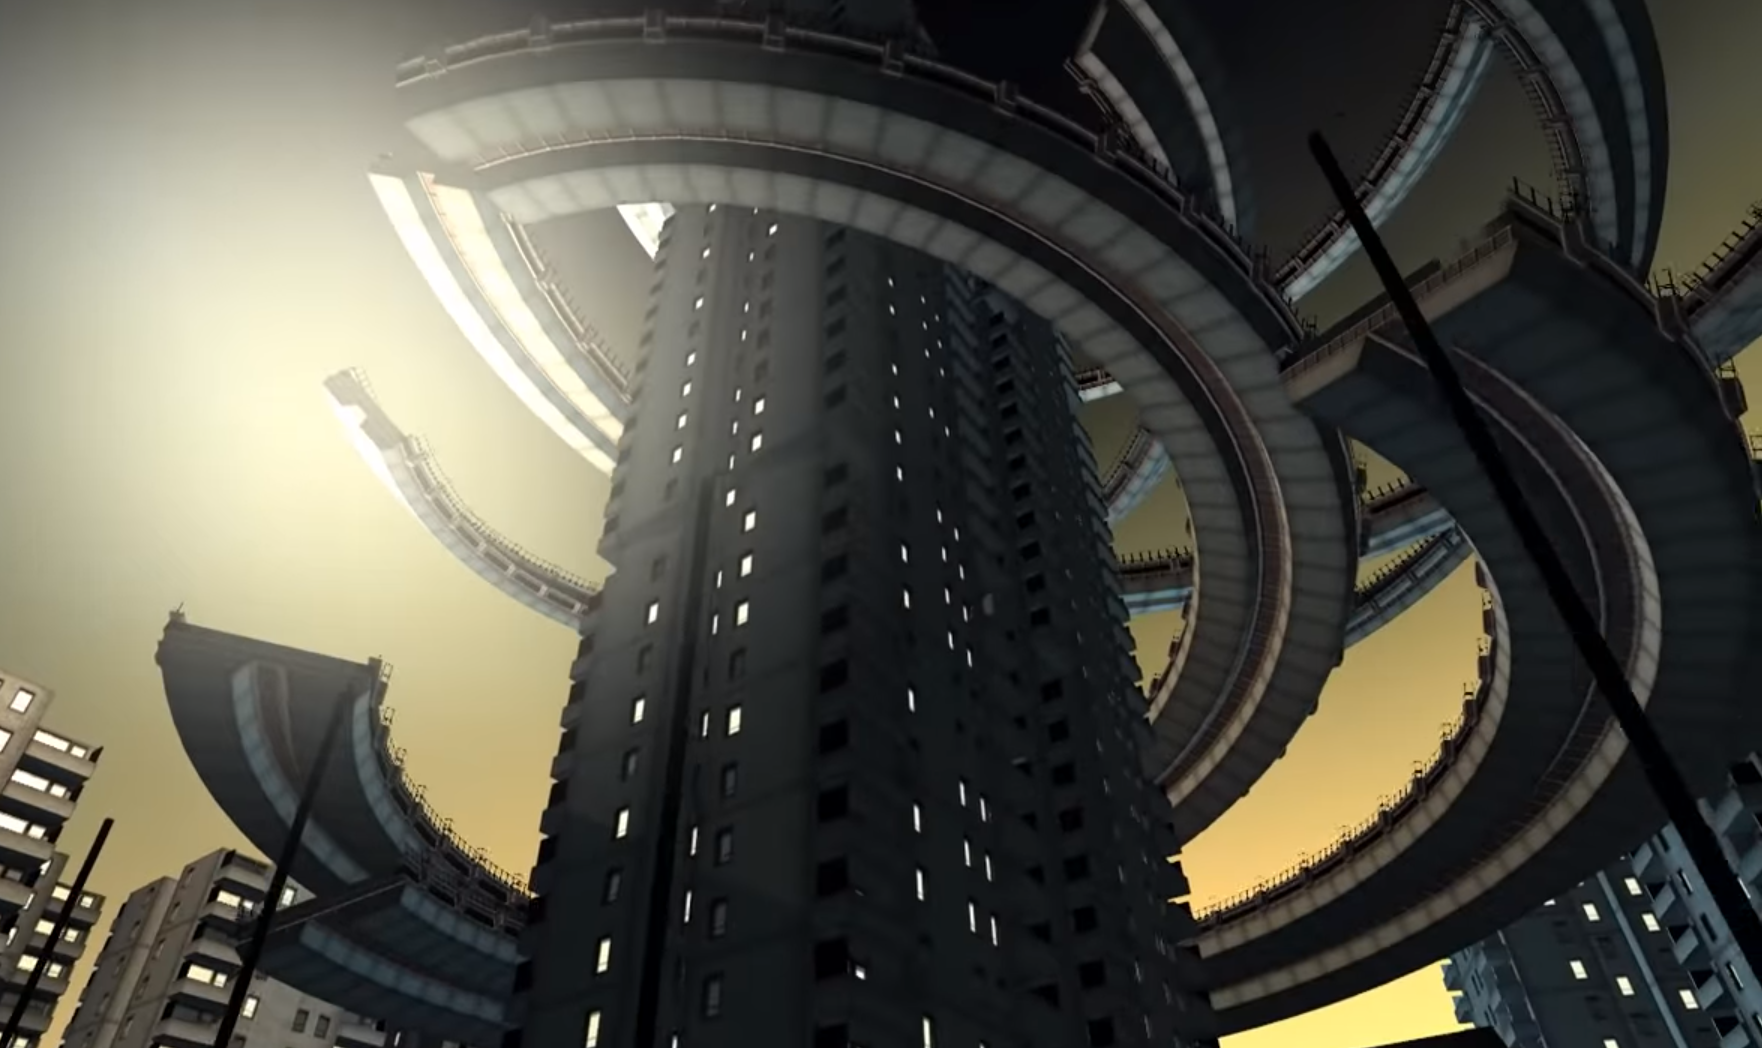
\includegraphics[width=10cm]{archivos/fr-041-debris}
	\caption{Farbrausch 41: Debris}
	\label{fig:debris}
\end{figure}

Además, en el año 2004 un subgrupo dentro de Farbrausch, denominado \emph{.theprodukkt}, lanzó \emph{.kkrieger}, un juego de disparos en primera persona que ocupaba tan sólo 96kB. Este pequeño tamaño se consiguió mediante el uso de generación procedural para las texturas y el uso de formas básicas (cubos, esferas...) combinados y deformados para los modelos. El juego [\ref{fig:kkrieger}] recibió distintos premios y fue alabado por la comunidad.\\

\begin{figure}[h]
	\centering
	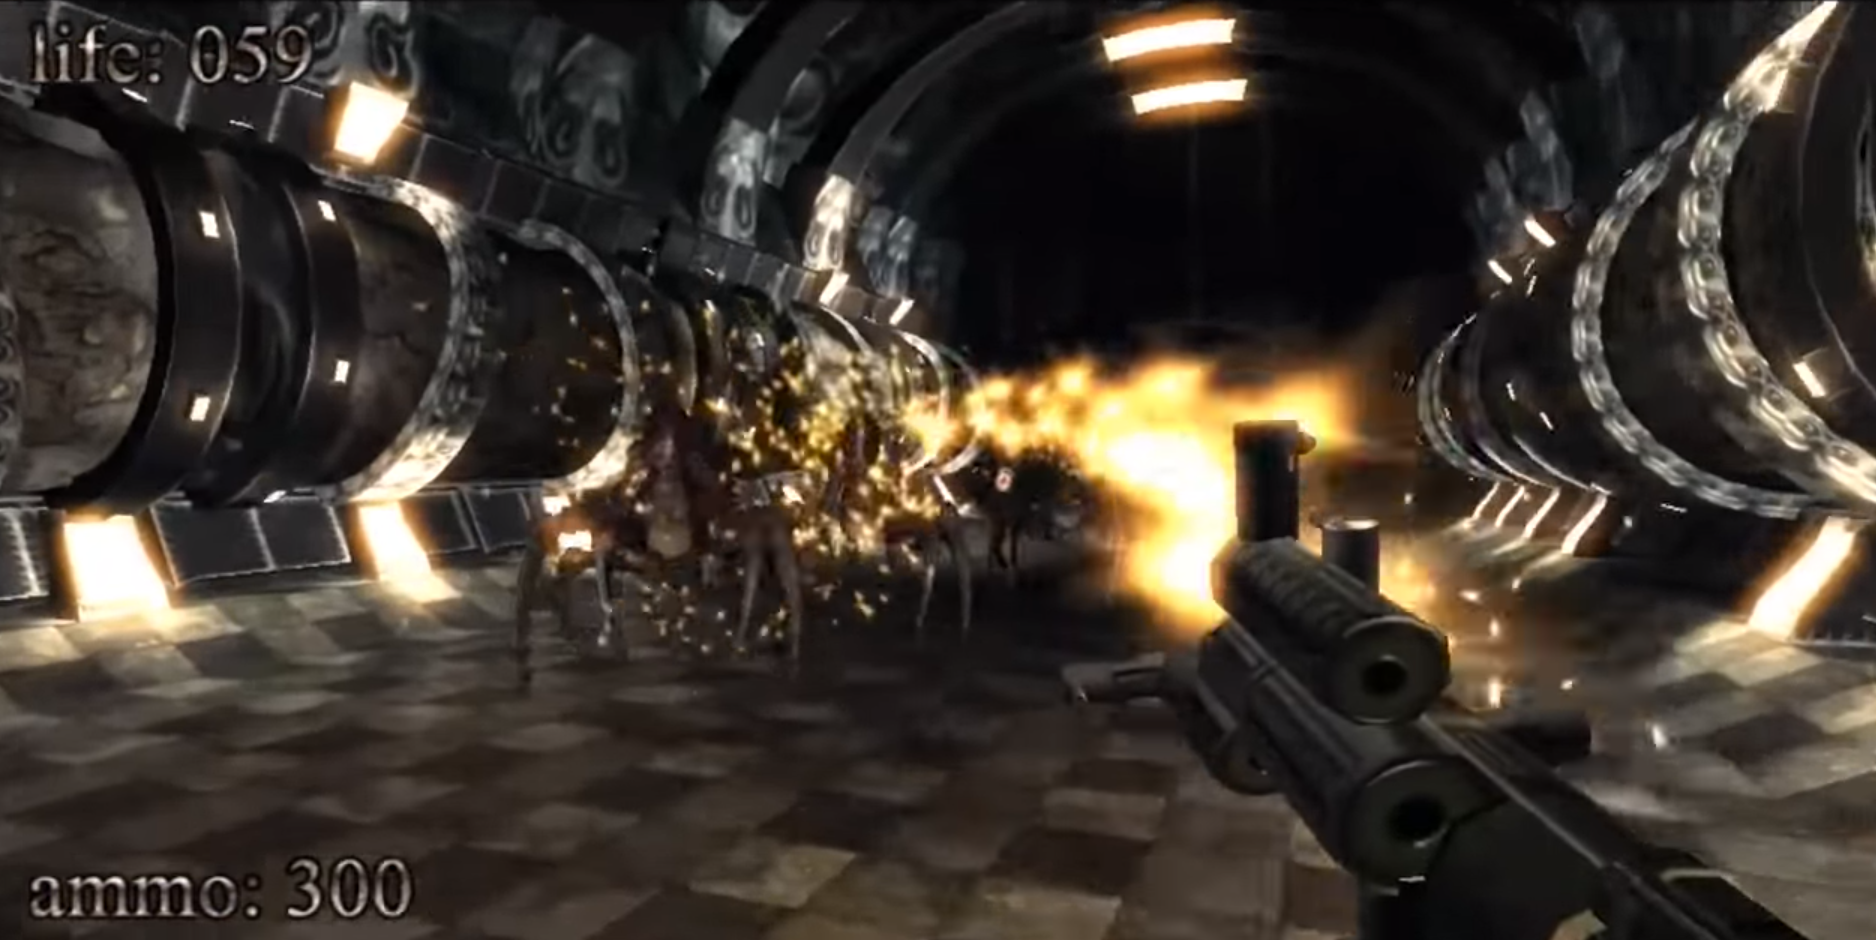
\includegraphics[width=10cm]{archivos/kkrieger}
	\caption{Videojuego de 96kB: .kkrieger}
	\label{fig:kkrieger}
\end{figure}

El grupo sigue en activo y siguen produciendo obras de gran calidad, contando con más de diez productos que han recibido primeros premios en distintas competiciones. En general, sus demos tienden a proseer una temática bastante urbana o robótica, con un cierto aire post-apocalíptico.
Sin embargo, su capacidad, imaginación y variedad de contenido [\ref{fig:magellan}] nunca deja de sorprender.

\begin{figure}[h]
	\centering
	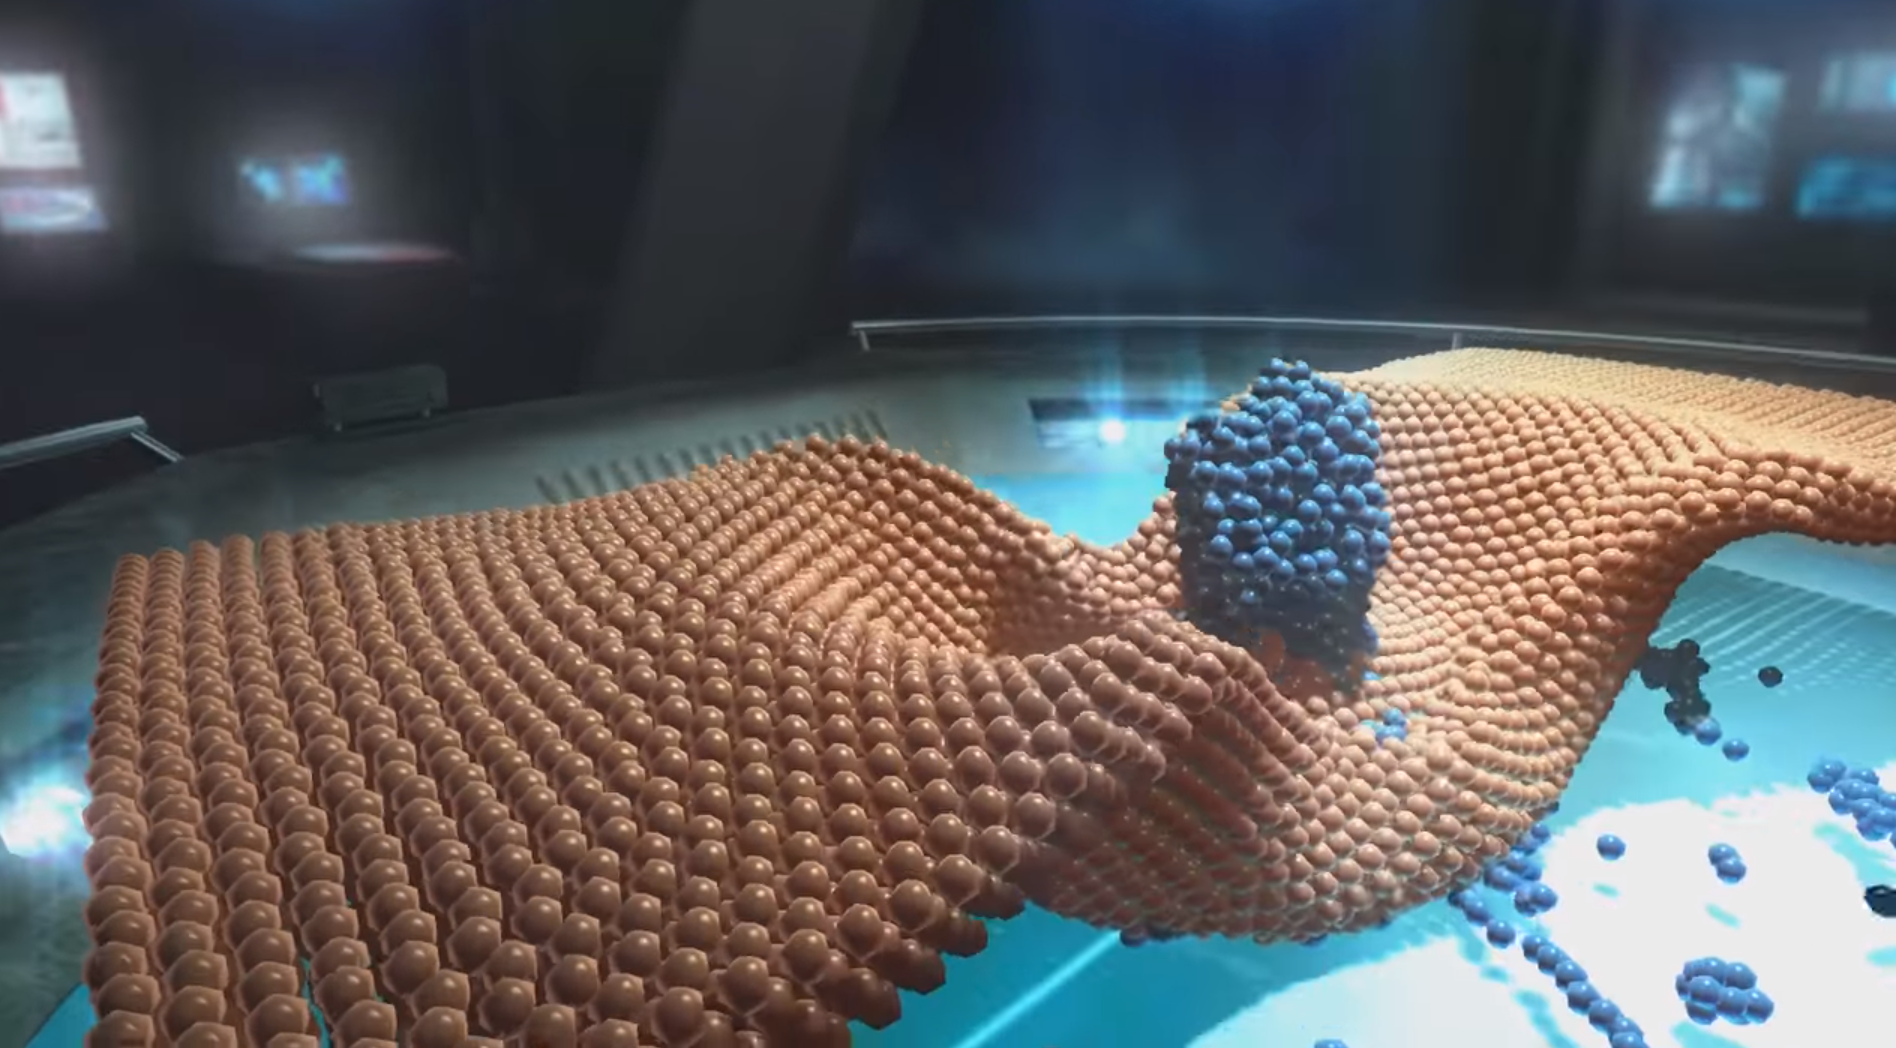
\includegraphics[width=10cm]{archivos/fr-063-magellan}
	\caption{Farbrausch 63: Magellan}
	\label{fig:magellan}
\end{figure}

%http://www.farbrausch.de/index.py https://en.wikipedia.org/wiki/Farbrausch
%https://en.wikipedia.org/wiki/Future_Crew https://demozoo.org/groups/357/
%http://www.popsyteam.org https://en.wikipedia.org/wiki/Very_Important_Party
%https://en.wikipedia.org/wiki/Equinox_(Atari_demogroup) https://equinox.planet-d.net/atari.html
%https://demozoo.org/groups/18871/

\section{Influencia de la demoscene en la industria}

La \emph{demoscene} siempre se ha mantenido de forma discreta. Algunas de las razones de que esto sea así se han listado anteriormente, como el hecho de que hace una gran cantidad de conocimiento y pasión para poder participar de forma activa en la \emph{demoscene}. Sin embargo, esto no ha impedido dejar su huella en la industria informática, especialmente en la del videojuego.\\

hablar de john carmack, del creadro del spore y ay dios me duele la vida no quiero escribir mas que os den chao

%Importantes para la historia:
%http://widerscreen.fi/assets/reunanen-wider-1-2-2014.pdf
%http://www.oldskool.org/demos/explained/demo_history.html
%https://web.archive.org/web/20170726063815/http://tomaes.32x.de/text/faq.php#2.3.

%Elevated y otras demos por el estilo

%https://web.archive.org/web/20170726063815/http://tomaes.32x.de/text/faq.php
%http://www.oldskool.org/demos/explained/demo_history.html

%http://www.oldskool.org/demos/explained/demo_reference.html

%http://www.demoscene.info
%http://www.pouet.net/index.php
%https://en.wikipedia.org/wiki/Assembly_(demoparty)
%https://en.wikipedia.org/wiki/Demoscene

%http://widerscreen.fi/numerot/2014-1-2/crackers-became-us-demosceners/
%http://www.oldskool.org/demos/explained/demo_pages.html
%ftp://ftp.hornet.org/pub/demos/info/demonews/1998/demonews.150

%http://www.farbrausch.de/index.py 
%https://en.wikipedia.org/wiki/Farbrausch
%https://en.wikipedia.org/wiki/Future_Crew 
%https://demozoo.org/groups/357/
%http://www.popsyteam.org 
%https://en.wikipedia.org/wiki/Very_Important_Party
%https://en.wikipedia.org/wiki/Equinox_(Atari_demogroup) 
%https://equinox.planet-d.net/atari.html
%https://demozoo.org/groups/18871/